\documentclass[UTF8]{ctexart}
\usepackage{geometry}
\usepackage{bookmark}
\usepackage{hyperref}
\geometry{a4paper,scale=0.8}
\usepackage{ctex}
\usepackage{booktabs}
\usepackage{array}
\usepackage{fancyhdr}
\usepackage{amsmath}
\pagestyle{fancy}
\fancyhf{}
\renewcommand\footrulewidth{1pt}
\lhead{\textit{王铠泽}}
\rhead{\textit{PB18020766}}
\chead{\href{mailto:volar@mail.ustc.edu.cn}{\textit{volar@mail.ustc.edu.cn}}}
\rfoot{\href{http://en.ustc.edu.cn/}{\textit{中国科学技术大学}}}
\lfoot{\textit{\today}}
\usepackage{graphicx}
\usepackage{float}
\usepackage{subfigure}
\fancyfoot[C]{\textbf{\textit{\thepage}}}

\begin{document}

	\centering\textbf{\LARGE{计算物理A第十三次作业}}
	
	
	\textit{王铠泽\qquad PB18020766}
	
		
	\section{实现目标}
	
	\begin{flushleft}
		用$ Metropolis-Hasting $抽样方法计算积分:
	\end{flushleft}
	
	$$I=\int_{0}^{\infty}(x-\alpha\beta)^2f(x)dx=\alpha\beta^2$$
	
	$$f(x)=\frac{1}{\beta\Gamma(\alpha)}{\left( \frac{x}{\beta}\right)}^{\alpha-1}exp(\frac{-x}{\beta})$$
	
	\begin{flushleft}
		设积分的权重函数为:$p(x)=f(x)$和$p(x)={(x-\alpha\beta)}^2f(x)$,给定参数$\alpha,\beta$,并用不同的$\gamma$值,分别计算积分,讨论计算精度和效率。
	\end{flushleft}
	
	
	
	\section{实现方法}
	
	\begin{flushleft}
		按 $p(x)$ 为平稳分布来实现$ Metropolis-Hasting $抽样。
		
		设$T$与初态无关(即非对称的):$T_{ij}=T(x\rightarrow x')=T(x')=0.5 \,exp\frac{-x'}{\gamma}$
		
		设$x_0=1$, 抽样$x'=-\gamma lnR$, $R$ 为[0,1]上均匀分布的随机数,由此抽取在(0,$\infty$)上分布的$x'$。
		
		$$\frac{p_{j}T_{ji}}{p_iT_{ij}}\equiv r=\left( \frac{x'}{x_i}\right) ^{\alpha-1}exp[-(x'-x_i)/\beta]exp[(x'-x_i)/\gamma]$$
		
		最后按照$r$的大小来决定接受概率,得到下一步的$x_{i+1}$
		
$$x_{i+1}=
\begin{cases}
	x'& {R'<min(1,r)}\\
	x_i&{R'>min(1,r)}
\end{cases}$$

其中$R'$为[0,1]上均匀分布的随机数

最后只需要用求和近似积分:

$$I=\frac{1}{N-m}\sum_{i=m+1}^{N}(x_i-\alpha\beta)^2$$

其中$m$是为了去除前面热化阶段引入的参数,本次实验中,取$m=\frac{N}{10}$。

本实验中,取 $\alpha=2,\beta=1$,调整不同$\gamma$来讨论精度和效率。

	\end{flushleft}
	
	\section{程式说明}
	
		\begin{itemize}
			\item metropolis\_1.c
			
			这是一个对于用于生成对于$N=10^{6}$步数的$Metropolis$抽样计算积分的误差评估的程序。其输出为不同$\gamma$值下面的积分误差,并且输入到文件中。注意到,循环中的$\gamma$范围根据需要可以修改。
			
			\item metropolis\_2.c
			
			这是一个对于用于生成对于不同步数$N=10^{1}\sim10^{7}$步数的$Metropolis$抽样计算积分的误差评估的程序。其输出为不同$\gamma$值下面的积分误差,并且输入到文件中。注意到,循环中的$\gamma$范围根据需要可以修改。本次实验中取$\gamma$值为0.2,1.4,4.0。
			
			
			\item rdm.h
			
			这是一个包含了使用16807产生器生成指定长度的$[0,1]$上均匀分布随机数函数的头文件。
			
			\subitem void rdm(int N,double *x,int method)
			
			该函数将输入的指针$x$对应的长度为$N$的数组用$[0,1]$上的随机数填满。method是关于初始种子的选择。method=0:默认种子;method=1,时间种子。
			
			\item time\_seed(gamma range).txt
			
			对于括号内标识的$\gamma$取值范围对应使用的时间种子文件。注意在程式中生成随机数时,一组随机数使用时间种子,另一组采用默认种子值($I$=1)。16807产生器抽样时对应的时间种子数据(每次1个种子)。调用多少次16807生成器就生成多少个数据记录。每一个分布对应的种子已经手动加上对应的实验了。种子产生公式如下:
			
		
				
			\begin{figure}[H]
				\centering  %图片全局居中
				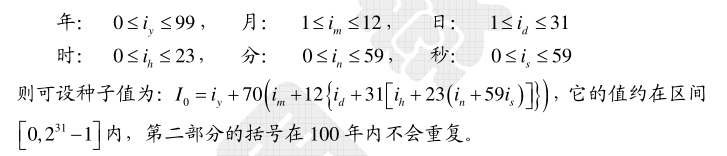
\includegraphics[width=4in]{1.png}
			\end{figure}
					
		\end{itemize}
	
	
	\section{计算结果}
	
	\subsection{不同$\gamma$参数值对于积分的影响}
	
	\begin{flushleft}
		取$N=10^{6}$,调节$\gamma$的取值,使得其取值落在$0\sim10^{4}$范围,然后做出误差-$log(\gamma)$图像如下:
		
			\begin{figure}[H]
				\centering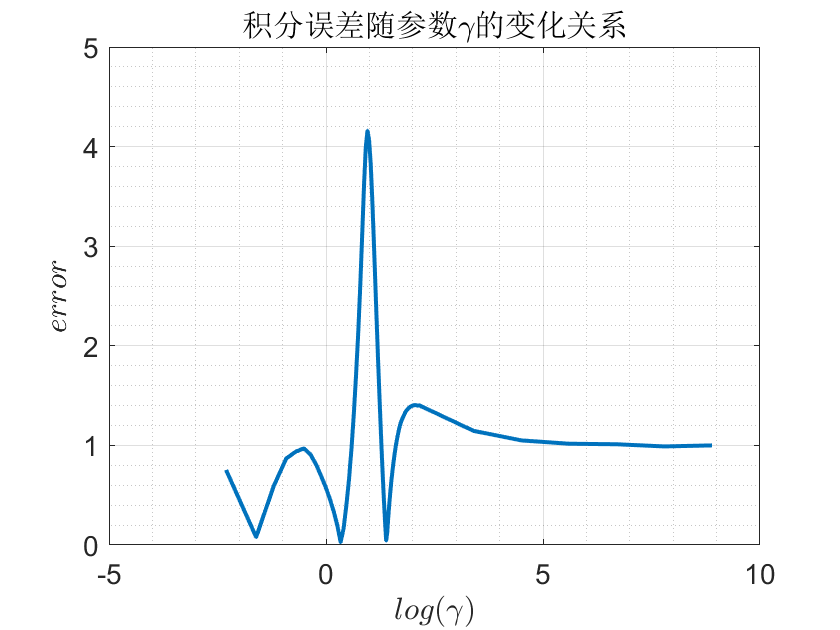
\includegraphics[width=4in]{gamma_error}
				\caption{error-log($\gamma$)图线}
				\end{figure}
		可以观察到基本可以认为在$\gamma>0$的范围内,积分误差会出现三个极小值,分别是$0.2,1.4,4.0$。在其附近更加精确的采点绘出的图像如下:
		
		\begin{figure}[H]
			\centering  %图片全局居中
			\subfigure[$\gamma\in(1.2,4.2)$]{
				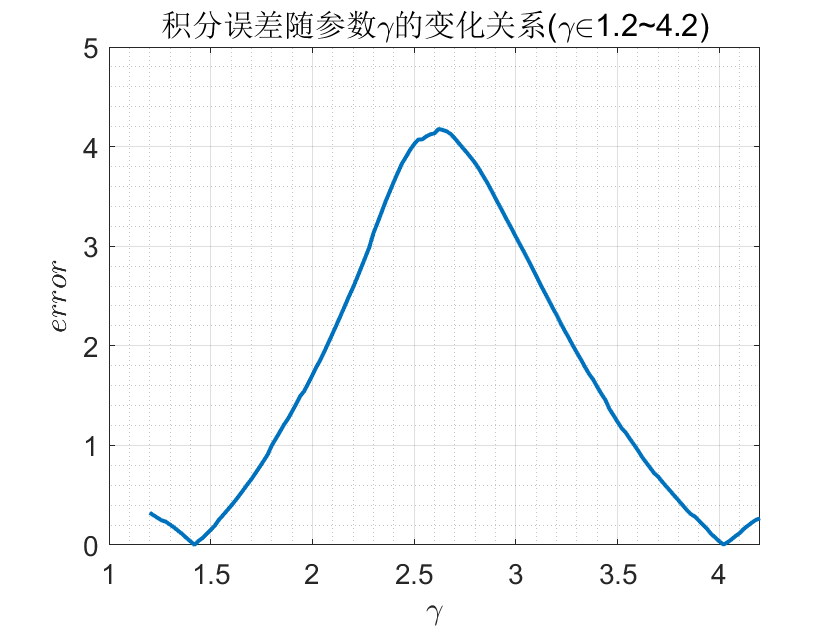
\includegraphics[width=0.45\textwidth]{gamma1.png}}
			\subfigure[[$\gamma\in(0,0.4)$]{
				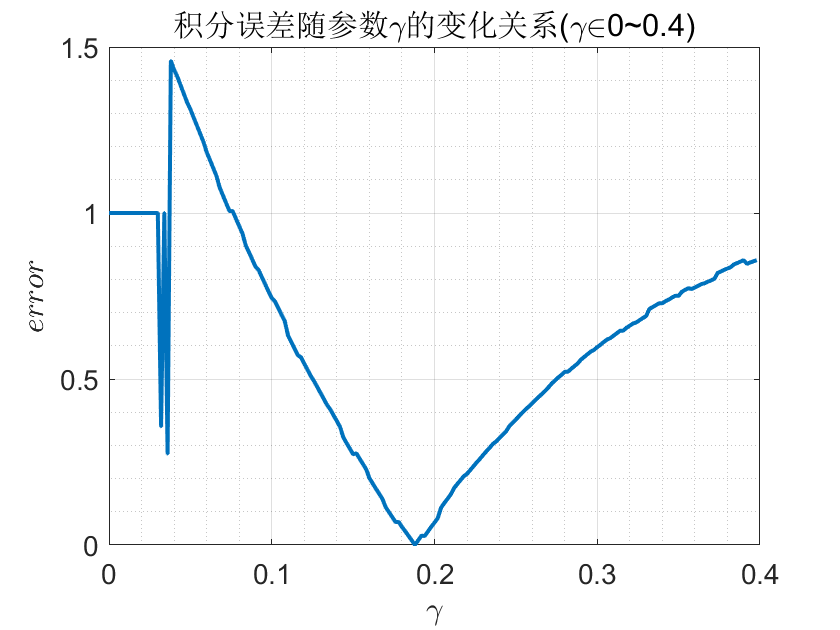
\includegraphics[width=0.45\textwidth]{gamma2.png}}
			\caption{误差随步数$N$变化曲线}
		\end{figure}
		
		可以非常明确的确定这就是三个极小值点,能够得到最理想的积分误差。从图线中可以看出,\textbf{积分误差对于$\gamma$的依赖性非常明显},选择不合适的$\gamma$很可能会导致积分误差非常大(即使已经走了很大的步数)。有趣的是在很大的$\gamma$下,误差基本稳定在1左右。不过这也是可以理解的:$\gamma$是$T_{ij}$抽样时对应的指数分布的参数,\textbf{当$\gamma$大到一定程度时,指数分布下降得非常快,基本只剩下$0$附近的点被抽到,这等价于很小的步进距离,这当然是不合适的},要经过相当长的步长才能达到平稳分布。同理,\textbf{太小的$\gamma$	也是不合适的,因为这样每一步都走的很大,很难以到达合适的平衡位置},这在图上也有所体现。
	\end{flushleft}
	
	
	\subsection{不同步数$N$对积分误差的影响}
	
	取在上述分析中误差的极小值点来进行步数依赖的分析。
	\setlength{\tabcolsep}{14mm}{
	\begin{table}[H]
			\centering
			\begin{tabular}{@{}ll@{}}
				\toprule
				积分步数$N$&绝对误差$\epsilon$ \\ \midrule
				10	&	1.000000\\
				100		&0.192531\\
				1000	&	0.137306\\
				10000	&	0.028388\\
				100000	&	0.099934\\
				1000000	&	0.099932\\
				10000000&		0.087569\\\bottomrule
			\end{tabular}
		\caption{$\gamma=0.2$时的积分误差表}
		\end{table}}
	
	\setlength{\tabcolsep}{14mm}{
		\begin{table}[H]
			\centering
			\begin{tabular}{@{}ll@{}}
				\toprule
				积分步数$N$&绝对误差$\epsilon$ \\ \midrule
			 10	&	0.585176\\
			100	&	0.269133\\
			1000&		0.203556\\
			10000&		0.043600\\
			100000&		0.024212\\
			1000000&		0.040619\\
			10000000&		0.032623\\\bottomrule
			\end{tabular}
			\caption{$\gamma=1.4$时的积分误差表}
	\end{table}}

	\setlength{\tabcolsep}{14mm}{
		\begin{table}[H]
			\centering
			\begin{tabular}{@{}ll@{}}
				\toprule
				积分步数$N$&绝对误差$\epsilon$ \\ \midrule
			 10	&	1.482793\\
			100	&	0.905431\\
			1000&		0.469053\\
			10000&		0.001988\\
			100000&		0.067546\\
			1000000&		0.030883\\
			10000000&		0.040191
								\\\bottomrule
			\end{tabular}
			\caption{$\gamma=4.0$时的积分误差表}
	\end{table}}

	\begin{flushleft}
		可以看出,当$N$较小的时候,误差很大,随着$N$增大,误差减小,并且后面误差随着$N$的增大几乎不会出现量级上的变化,比较稳定,这时候想要加大精度,可能要再走很多步,说明增大步数并不能非常有效地提高精度。以步数的对数作为横坐标,误差作为纵坐标,做出的曲线图如下:
		
		\begin{figure}[H]
					\centering  %图片全局居中
					\subfigure[$\gamma=0.2$]{
						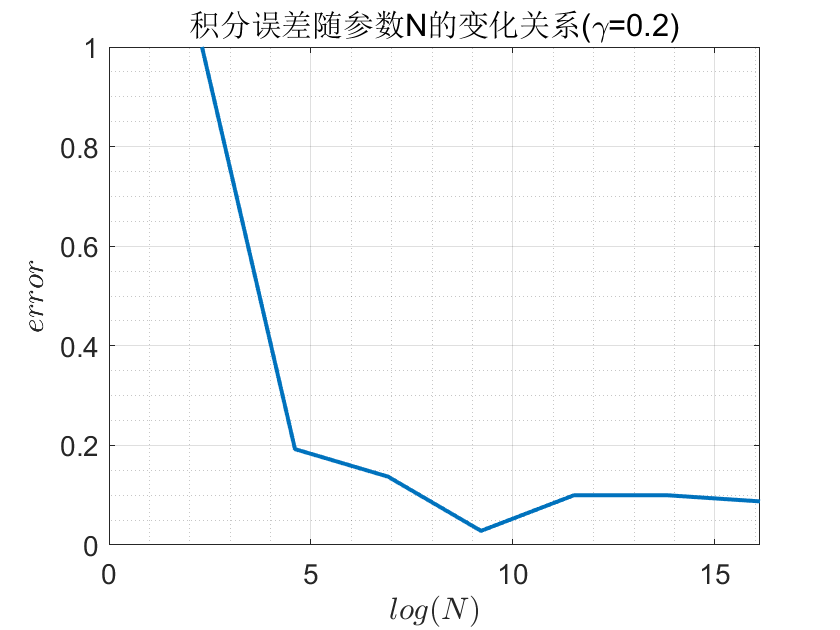
\includegraphics[width=0.45\textwidth]{02.png}}
					\subfigure[$\gamma=1.4$]{
						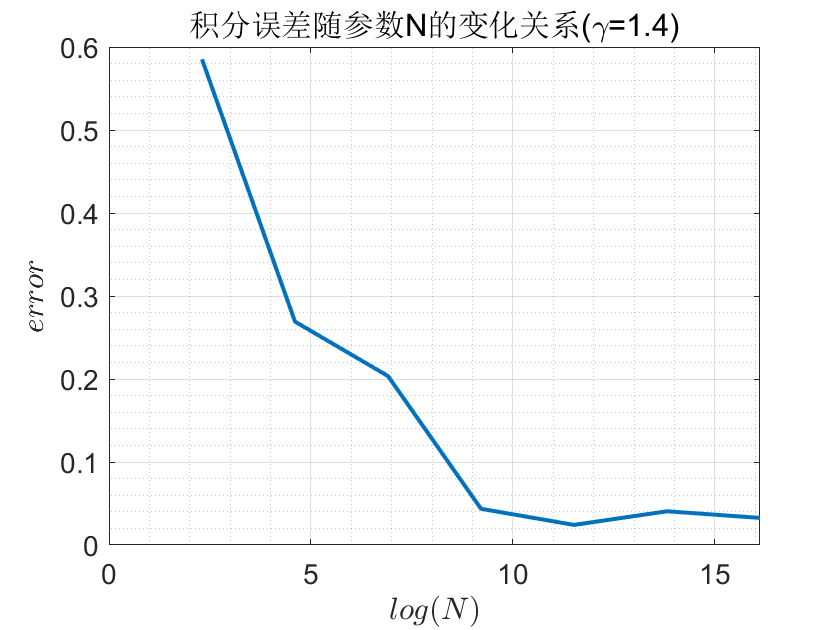
\includegraphics[width=0.45\textwidth]{14.png}}
					\subfigure[$\gamma=4.0$]{
						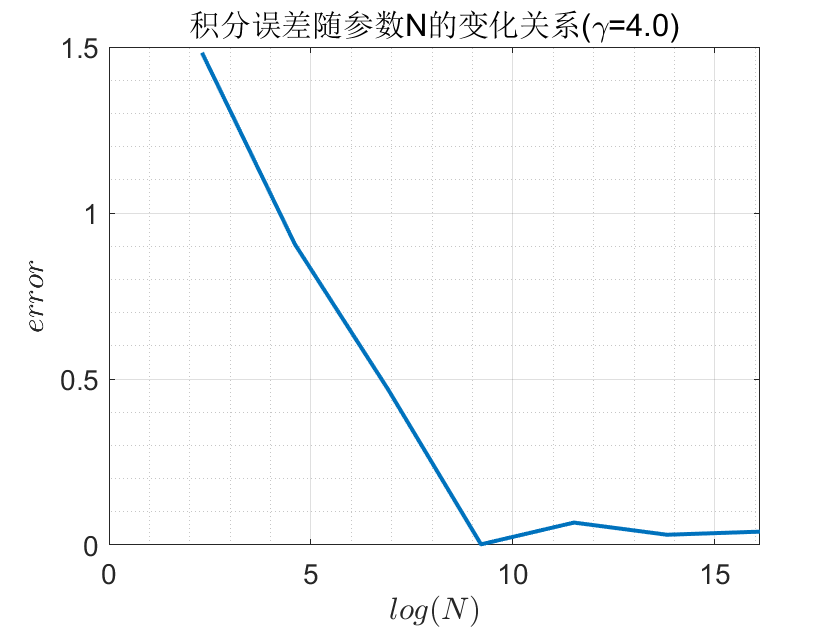
\includegraphics[width=0.45\textwidth]{40.png}}
					\caption{误差随步数$N$变化曲线}
				\end{figure}
	从曲线上更加直观地看出,最后随着步数增加误差和步数之间并没有很明显的单调递减关系,而是变得逐渐平缓,控制在0.1的量级。
	
	\end{flushleft}


%	\begin{figure}[H]
%	\centering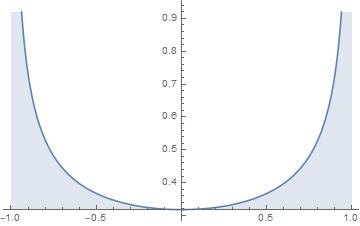
\includegraphics[width=2in]{1.jpg}
%	\caption{something}\label{fig:1}
%	\end{figure}
		
%	\begin{figure}[H]
%		\centering  %图片全局居中
%		\subfigure[name1]{
%			\label{Fig.sub.1}
%			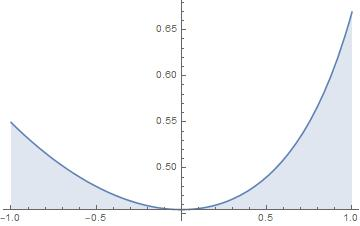
\includegraphics[width=0.45\textwidth]{2.jpg}}
%		\subfigure[name2]{
%			\label{Fig.sub.2}
%			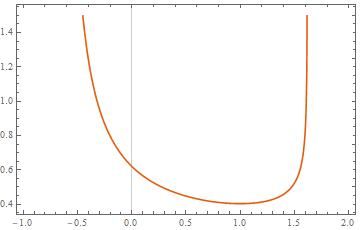
\includegraphics[width=0.45\textwidth]{3.jpg}}
%		\caption{Main name}
%		\label{Fig.main}
%	\end{figure}

	\section{总结}

	\begin{itemize}
		\item 本次实验通过$Metropolis$抽样实现积分的计算,选择合适的参数值,能够得到较为理想的模拟结果
		\item 可以发现$Metropolis$抽样对于步进矩阵$T$的选择有很高的要求,一个合适的$T$矩阵应该使得每一步的步长不能太长也不能太短,这样才能在尽可能少的步数到达热平衡态,得到我们所要的重要抽样分布。
	\end{itemize}

\end{document}